\documentclass[nobib]{tufte-handout}

\title{Lecture 7: The max-flow min-cut theorem $\cdot$ 1MA020}

\author[Vilhelm Agdur]{Vilhelm Agdur\thanks{\href{mailto:vilhelm.agdur@math.uu.se}{\nolinkurl{vilhelm.agdur@math.uu.se}}}}

\date{14 November 2023}


%\geometry{showframe} % display margins for debugging page layout

\usepackage{graphicx} % allow embedded images
  \setkeys{Gin}{width=\linewidth,totalheight=\textheight,keepaspectratio}
  \graphicspath{{graphics/}} % set of paths to search for images
\usepackage{amsmath}  % extended mathematics
\usepackage{booktabs} % book-quality tables
\usepackage{units}    % non-stacked fractions and better unit spacing
\usepackage{multicol} % multiple column layout facilities
\usepackage{lipsum}   % filler text
\usepackage{fancyvrb} % extended verbatim environments
  \fvset{fontsize=\normalsize}% default font size for fancy-verbatim environments

\usepackage{color,soul} % Highlights for text

% Standardize command font styles and environments
\newcommand{\doccmd}[1]{\texttt{\textbackslash#1}}% command name -- adds backslash automatically
\newcommand{\docopt}[1]{\ensuremath{\langle}\textrm{\textit{#1}}\ensuremath{\rangle}}% optional command argument
\newcommand{\docarg}[1]{\textrm{\textit{#1}}}% (required) command argument
\newcommand{\docenv}[1]{\textsf{#1}}% environment name
\newcommand{\docpkg}[1]{\texttt{#1}}% package name
\newcommand{\doccls}[1]{\texttt{#1}}% document class name
\newcommand{\docclsopt}[1]{\texttt{#1}}% document class option name
\newenvironment{docspec}{\begin{quote}\noindent}{\end{quote}}% command specification environment

\include{mathcommands.extratex}

\begin{document}

\maketitle% this prints the handout title, author, and date

\begin{abstract}
\noindent
Continuing our exploration of things that can be done with weighted graphs, we move on to considering \emph{flows} in weighted directed graphs, which model things like traffic flows. We see the connection between these and edge cuts of graphs, and prove the Ford-Fulkerson theorem.
\end{abstract}

In our exercises, we saw this figure:
\begin{figure}
    \centering
    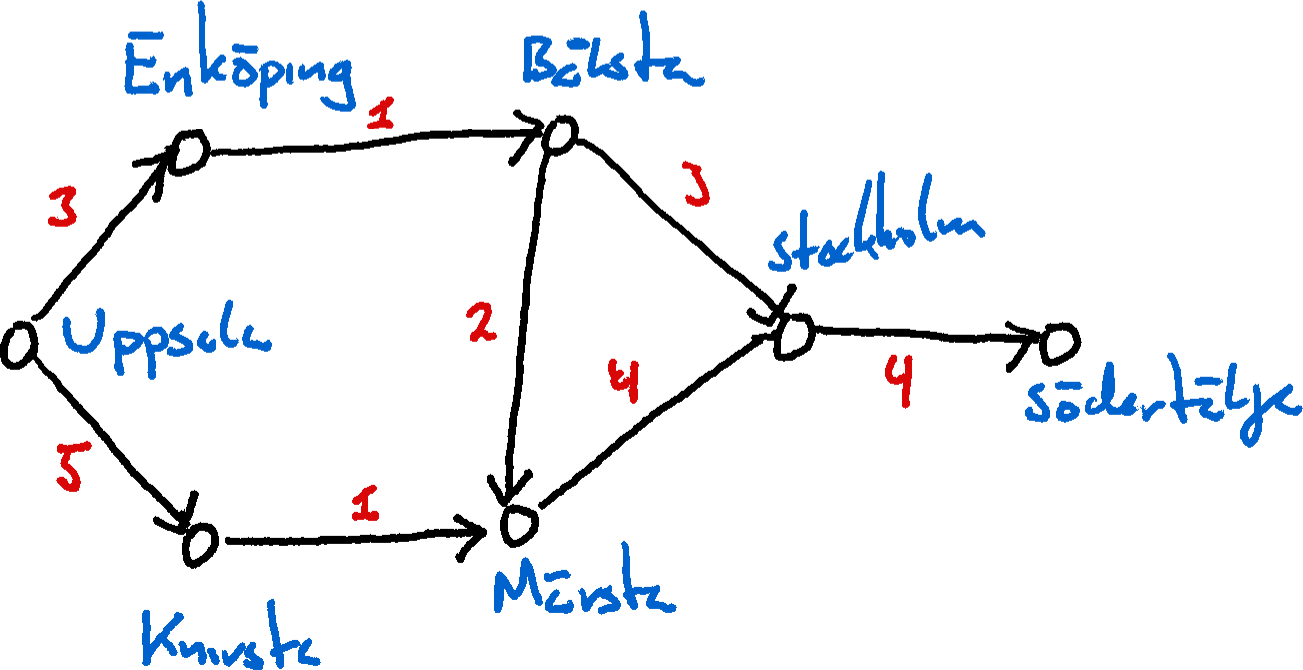
\includegraphics[width=0.85\textwidth]{graphics/L5_exc_MSTs_etc/train_network_flow.png}
    \caption[][0cm]{A hypothetical graph modelling public transport flow from Uppsala to Södertälje.}
    \label{fig:uppsala_stockholm_traffic}
  \end{figure}

  If we interpret the edge-weights as how many thousands of passengers can travel the route per hour, it makes sense to ask the question of how many can travel from Uppsala to Södertälje per hour. Intuitively, it is clear that the answer must be two thousand, because the traffic is bottlenecked by the Enköping-Bålsta and Knivsta-Märsta connections -- the fact that five thousand per hour can get from Uppsala to Knivsta doesn't help at all, and upgrading the Bålsta-Stockholm route wouldn't improve things.

  Let us now turn these intuitive considerations into actual rigorous mathematics. First, let us define the graphs we are working on:

  \begin{definition}
    A \emph{weighted directed graph} $G$ consists of a directed graph $(V,E)$ and a weight function $w: E \to \R$. For it to be a \emph{flow network} we additionally require that all weights be positive, that there be a distinguished \emph{source} vertex $s$ and \emph{sink} vertex $t$, and that whenever $u \to v$ is an edge, $v \to u$ is not also an edge.\sidenote[][-3cm]{Recall that in general, it is allowed in a simple directed graph to have both the edge $u\to v$ and the edge $v\to u$ -- what is not allowed is multiples of the same edge, or loops. In this case, the restriction of not having such back-and-forth edges is not a genuine restriction, however: If we have such a pair of edges, we can get an equivalent flow network by introducing a ``dummy vertex'' in the middle of one of the edges, as in Figure \ref{fig:dummy_edge}.}

    \begin{marginfigure}
        \centering
        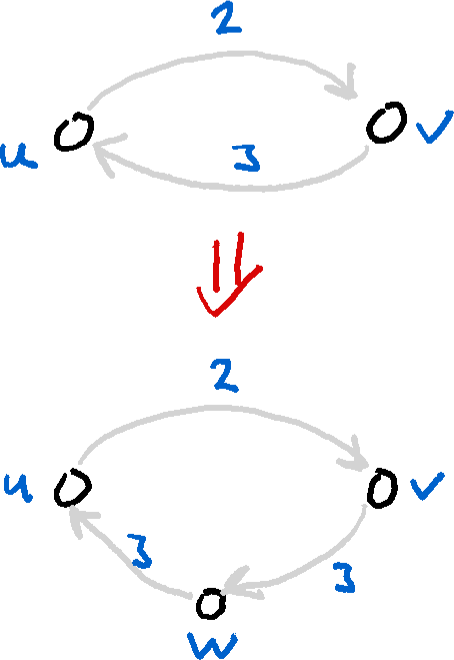
\includegraphics[width=0.5\textwidth]{graphics/L7_flows/dummy_edge.png}
        \caption{Subdividing an edge using a dummy vertex, to get around the restriction that there be no back-and-forth edges.}
        \label{fig:dummy_edge}
    \end{marginfigure}

    We define a \emph{capacity function} $c: V\times V \to [0,\infty)$ by that $c(v,v') = w(v\to v')$ whenever $v\to v'$ is an edge of $G$, and $c(v,v') = 0$ otherwise.
  \end{definition}

  These flow graphs define the capacity of the network to handle traffic. Next, let us define the actual \emph{flows}, which are the possible actual traffic situations. There are two natural constraints these should satisfy:
  \begin{enumerate}
    \item The flow through an edge can't be greater than the actual capacity of the edge, so we aren't putting more cars on the road than will actually fit.
    \item Other than the source and the sink nodes, where we imagine vehicles are entering and exiting the graph, the flow into a vertex must equal the flow out of it. Trains do not magically vanish, nor do they appear out of nowhere or teleport.
  \end{enumerate}

  \begin{definition}
    A \emph{flow} on the flow network $G$ with capacity function $c$ is a function $f: V \times V \to [0,\infty)$ which satisfies
    \begin{enumerate}
        \item the \emph{capacity constraint} that
        $$f(v, v') \leq c(v, v')\qquad \forall v, v' \in V,$$
        \item and the \emph{conservation constraint}
        $$\sum_{w \in V} f(w, v) = \sum_{u \in V} f(v, u)$$
        whenever $v \in V \setminus \{s,t\}$.
    \end{enumerate}

    The \emph{value} of a flow, denoted by $\abs{f}$, is the net out-flow at the source, that is
    $$\abs{f} = \sum_{v \in V} f(s, v) - \sum_{w \in V} f(w, s).$$
\end{definition}

\begin{figure}
    \centering
    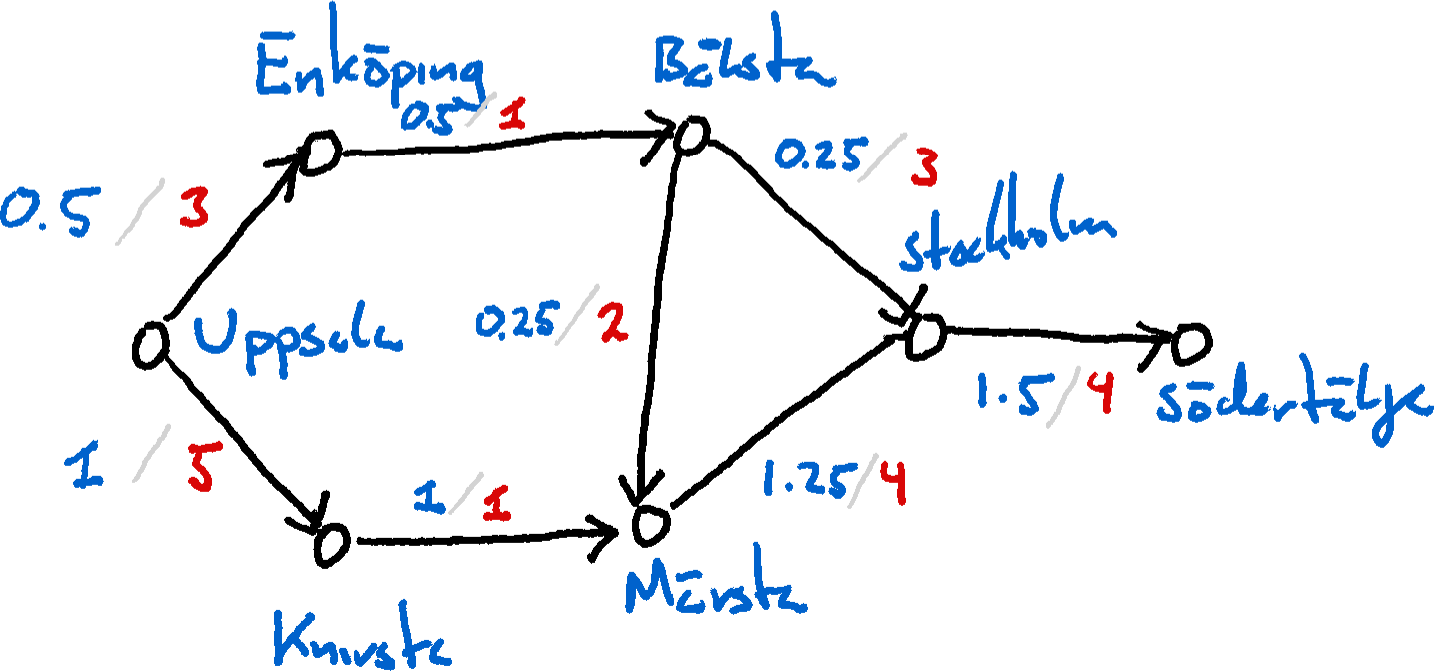
\includegraphics[width=0.9\textwidth]{graphics/L7_flows/flow.png}
    \caption[][0cm]{An example of a flow in the graph from Figure \ref{fig:uppsala_stockholm_traffic}. The weights of the edges are given in red, and the flows through them in blue. This flow has value $1.5$, which we can see both by computing the net out-flow from Uppsala and the net flow into Södertälje.}
    \label{fig:flow}
\end{figure}

\begin{remark}
    It follows from the conservation constraint that $\abs{f}$ is also equal to the net in-flow at the sink.\sidenote[][]{
        \begin{xca}
            Prove this.
        \end{xca}
    } Therefore, we can always assume that $\abs{f} \geq 0$, since if it were not, we could just swap the roles of $s$ and $t$.
\end{remark}

Having defined what we mean by a flow, let us next formalize the intuitive notion of a bottleneck in the graph.

\begin{definition}
    Let $G = (V,E,w,s,t)$ be a flow network with source $s$ and sink $t$. An \emph{s-t-cut} is a partitioning of $V$ into two sets $S, T$ such that $s \in S$ and $t \in T$. The \emph{capacity} of the cut is
    $$c(S,T) = \sum_{(v,v') \in S \times T} c(v,v') = \sum_{e \in E(S,T)} w(e).$$
\end{definition}

Considering our intuition about the bottlenecks, it should be clear that any flow from $s$ to $t$ has to at some point pass from $S$ into $T$, and so use some of the capacity of the cut. So the total flow cannot be greater than the capacity of the cut, that is, $\abs{f} \leq c(S,T)$ for any flow $f$ and any s-t-cut $S,T$.

In fact, it turns out that equality is only achieved in this inequality in the most extreme case.

\begin{lemma}\label{lemma:cut_equals_flowvalue_implies_maximal}
    Let $G$ be a flow network with a flow $f$ and an s-t-cut of $V$ into $S$ and $T$. If $\abs{f} = c(S,T)$, then $\abs{f}$ is maximal among all flows, and $c(S,T)$ is minimal among all s-t-cuts.

    \begin{proof}
        As we saw, for any other flow $f'$, we must have 
        $$\abs{f'} \leq c(S,T) = \abs{f},$$
        and so $f$ is maximal. Similarly, for any other s-t-cut $S', T'$ we have
        $$c(S,T) = \abs{f} \leq c(S',T')$$
        and so $S, T$ is minimal.
    \end{proof}
\end{lemma}

A central construction in the theory of flow networks is the \emph{residual network}, which as the name suggests encodes how much capacity is left over by a flow.

\begin{definition}
    Let $G$ be a flow network with capacity function $c$, and let $f$ be a flow on $G$. The \emph{residual capacity} $c_f$ is a function from $V\times V$ into $[0,\infty)$ defined by\sidenote[][]{Notice how we use the assumption that there are no back-and-forth edges in $G$ here -- otherwise the definition would not make sense.}
    $$c_f(u,v) = \begin{cases}
        c(u,v) - f(u,v)&\text{if }(u,v)\text{ is an edge in }G\\
        f(v,u)&\text{if }(v,u)\text{ is an edge in }G\\
        0&\text{otherwise.}
    \end{cases}$$
    
    The \emph{residual network} $G_f$ is the weighted directed graph which has an edge $u \to v$ whenever $c_f(u,v) > 0$, and this edge has weight $c_f(u,v)$ if so.

    \begin{figure}
        \centering
        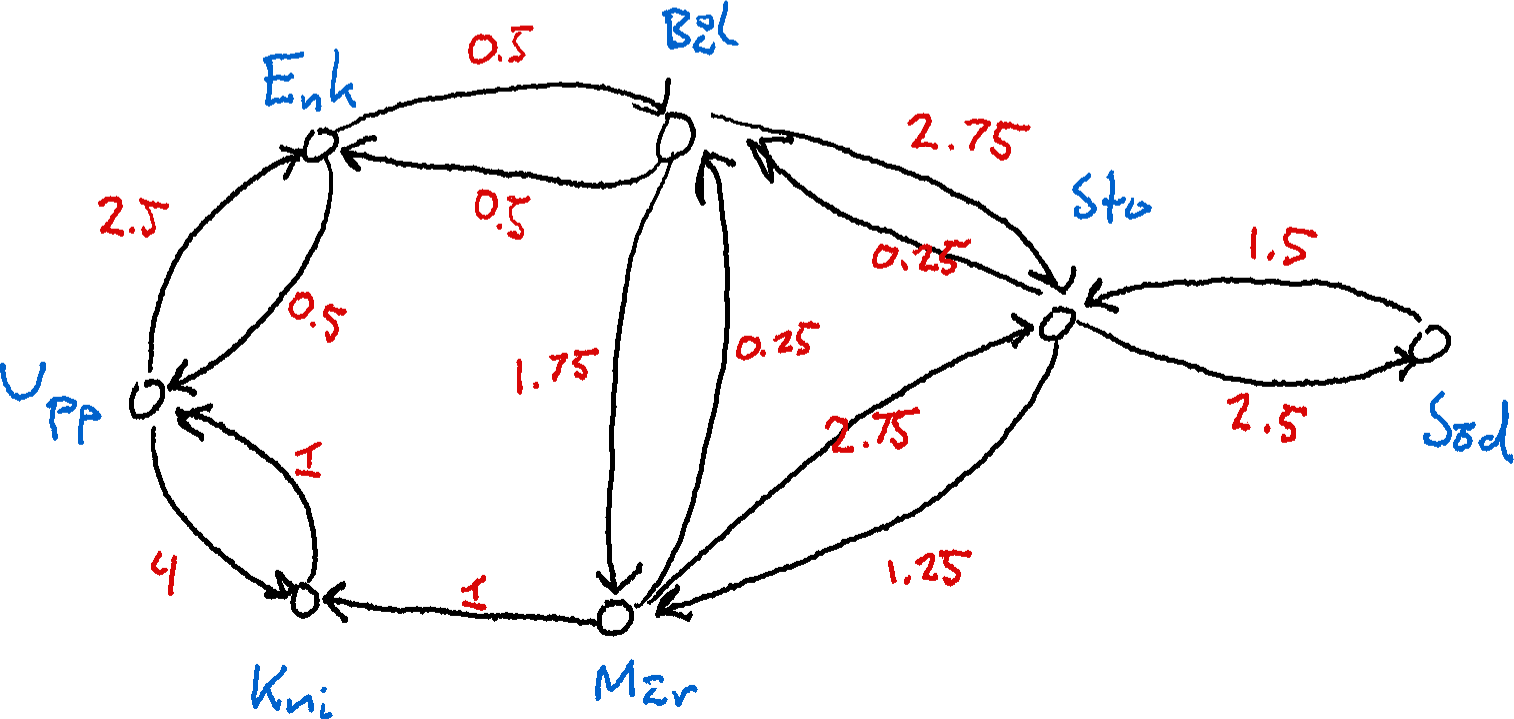
\includegraphics[width=0.8\textwidth]{graphics/L7_flows/residual_network.png}
        \caption[][0cm]{The residual network of the flow in Figure \ref{fig:flow}.}
        \label{fig:residual_network}
    \end{figure}

    We give an example of this in Figure \ref{fig:residual_network}, using the same flow network we have seen before.
\end{definition}

How can we use these residual networks to find ways to improve a flow? The idea is that a walk from the source to the sink in the residual graph will correspond to a way of improving the flow. However, so far we have only defined walks in undirected graphs, so let us define what we mean here.

\begin{definition}
    In any directed graph, a \emph{directed path} consists of a sequence of vertices $v_0\, v_1\, \ldots\, v_k$ and a sequence of edges $e_1\, e_2\, \ldots\, e_k$, such that edge $e_i$ points from $e_{i-1}$ to $e_i$. We also call such a path a $v_0$-$v_k$-path.

    If $G$ is a residual network, a directed path $P$ from $s$ to $t$ is called an \emph{augmenting path}, and it has \emph{residual capacity}
    $$c_f(P) = \min_{e\in E(P)} w(e).$$
\end{definition}

That these augmenting paths correspond precisely to ways to improve the flow is the content of our next lemma.

\begin{lemma}\label{lemma:can_augment_flows}
    Let $f$ be a flow in a flow network $G$ such that $G_f$ admits an augmenting path $P$. Then the flow $f'$ defined by
    $$f'(u,v) = \begin{cases}
        f(u,v) + c_f(P)&\text{if }(u,v)\text{ is an edge in }P\\
        f(u,v) - c_f(P)&\text{if }(v,u)\text{ is an edge in }P\\
        f(u,v)&\text{otherwise}
    \end{cases}$$
    satisfies $\abs{f'} > \abs{f}$.

    \begin{xca}
        This proof is mostly just a slightly tedious unpacking of the definitions, which is not very illuminating to do during a lecture, but useful to do yourself for learning the definitions. Therefore, we leave it as an exercise. Remember that there are three things you need to check:
        \begin{enumerate}
            \item The capacity constraint on $f'$,
            \item the conservation constraint on $f'$,
            \item and that $\abs{f'} > \abs{f}$. (Note that this is a \emph{strict} inequality!)
        \end{enumerate}
    \end{xca}
\end{lemma}

\begin{figure}
    \centering
    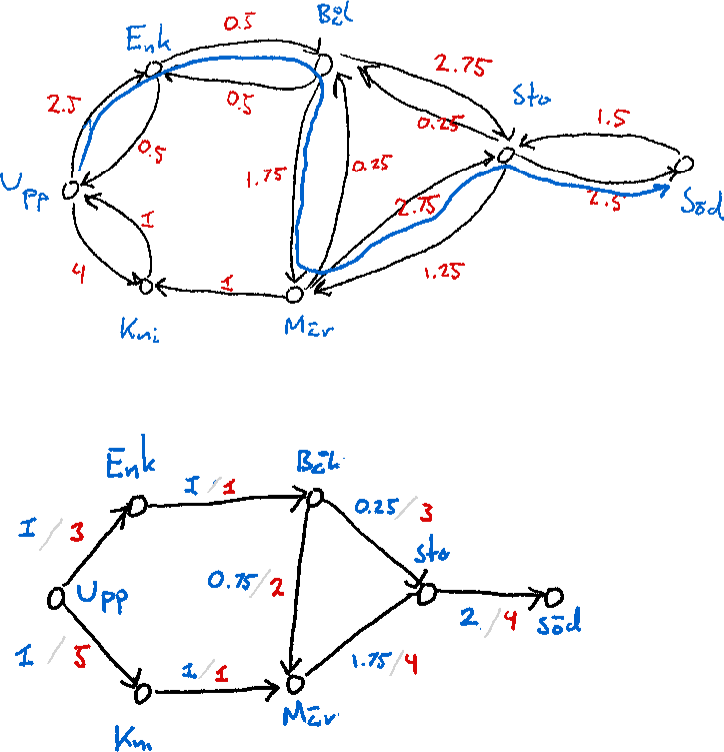
\includegraphics[width=0.8\textwidth]{graphics/L7_flows/augmenting_path.png}
    \caption[][0cm]{An augmenting path in the residual network of Figure \ref{fig:residual_network}, and the new flow $f'$ gotten from it.}
    \label{fig:augmenting_path}
\end{figure}

We see one example of improving a flow using an augmenting path in Figure \ref{fig:augmenting_path}.

Having now finally set up all the terminology and lemmata we need, we can finally state and prove the Ford-Fulkerson theorem.

\begin{theorem}
    Let $f$ be a flow on the flow network $G$. Then, the following are equivalent:
    \begin{enumerate}
        \item $f$ is a maximal flow,
        \item $G_f$ contains no augmenting path, and
        \item there is an s-t-cut $S,T$ with $\abs{f} = c(S,T)$.
    \end{enumerate}

    \begin{proof}
        That 3. implies 1. is precisely the content of Lemma \ref{lemma:cut_equals_flowvalue_implies_maximal}. To see that 1. implies 2., consider what the contrapositive of this implication is -- it is precisely that the existence of an augmenting path implies there is a higher-value flow, which is exactly Lemma \ref{lemma:can_augment_flows}.

        Therefore, the thing we need to show is that 2. implies 3. -- so assume $G_f$ does not contain an augmenting path,and let $S$ be the set of vertices that can be reached from $s$ by a directed path. Let $T = V \setminus S$. We want to show that these $S$ and $T$ are the desired s-t-cut with capacity equal to $\abs{f}$.
        
        By assumption $t\in T$, since otherwise there would be an augmenting path. We also see that every arrow $u \to v$ from $S$ to $T$ in $G$ must have its full capacity used by $f$, or there would be an arrow in $G_f$ from $u$ to $v$ corresponding to the unused capacity. Likewise, every arrow $u \to v$ from $T$ to $S$ must have a flow of zero, or there would be an arrow in the opposite direction in $G_f$. Therefore we must have $c(S,T) = \abs{f}$, as desired.
    \end{proof}
\end{theorem}

\begin{remark}
    Notice how this theorem does not actually say anything about the \emph{existence} of a maximal flow. For finite networks, however, we can do a bit of analysis-style reasoning to prove that a maximum flow must exist. The details of this are left as an exercise.
\end{remark}

\section{Exercises}

\begin{xca}
    Prove that for a finite flow network $G = (V,E,w)$ there always exists a maximal flow, because the set of possible flows can be seen as a compact subset of $\R^{\abs{E}}$, and the function sending $f$ to $\abs{f}$ is continuous.
\end{xca}

%\bibliography{references}
%\bibliographystyle{plainnat}

\end{document}
